% Created 2013-07-17 Wed 21:18
\documentclass[11pt]{article}
\usepackage[utf8]{inputenc}
\usepackage[T1]{fontenc}
\usepackage{graphicx}
\usepackage{longtable}
\usepackage{float}
\usepackage{wrapfig}
\usepackage{soul}
\usepackage{amssymb}
\usepackage{hyperref}
\usepackage{fontspec}
\usepackage[titletoc,page,title]{appendix}
\usepackage{biblatex}
\usepackage{metalogo}
\usepackage{graphicx}
\usepackage{moreverb}
\usepackage{fancyvrb}
\usepackage{fullpage}
\usepackage{setspace}
\usepackage{subfig}
\usepackage{algorithm}
\usepackage{algorithmic}
\usepackage[scientific-notation=true]{siunitx}
\usepackage{float}
\let\iint\relax % otherwise errors are thrown by amsmath. Defined in latexsym
\let\iiint\relax
\usepackage{amsmath}
\usepackage{hyperref}
\usepackage{tikz}
\usetikzlibrary{positioning}
\bibliography{summary}
\defaultfontfeatures{Mapping=tex-text}
\setromanfont[Ligatures={Common},Numbers={Lining}]{Linux Libertine}

\title{Time Delay Estimation in Gravitationally Lensed Photon Stream Pairs}
\author{\Large{Micha{\l} Staniaszek} \\\small{Supervisor: Peter Ti{\v{n}}o}}
\date{\today}

\begin{document}

\maketitle


this is the abstract

\section{Introduction}
\label{sec-1}

\begin{itemize}
\item explain the project in layman's terms
\end{itemize}
\section{Background}
\label{sec-2}

\begin{itemize}
\item Ideas behind the project
\item what it's useful for
\item what gravitational lensing and time delay are
\end{itemize}
\section{Photon Stream Simulation}
\label{sec-3}

  In the early stages of the project, we developed a subsystem which could be used
  to generate simulated photon stream data to use for the development and testing
  of the rest of the project. The only property of the photons which we are
  interested in is their arrival time at our capture device, so the simulator
  should produce some event vector $\Phi=\left[\phi_0,\dots,\phi_N\right], \phi_n
  \in \mathbb{R}$, where $\phi_n$ is the arrival time of the $n\text{th}$
  photon. In order to generate arrival times, we represent the source as some
  random variable $X$, which defines the average number of photons per unit time
  that arrive at the capture device, and whose varies according to the
  characteristic function of the source object.

  The characteristic function of $X$ is modelled as a non-homogeneous Poisson
  process (NHPP) with continuous function of time, $\lambda(t)$, known as the rate
  function. The rate function can be specified either by providing an expression
  which is a function of $t$, or by sampling from a randomly generated
  function. Random functions are constructed by uniformly distributing $M$
  Gaussians across the interval $\left[t_0,T\right]$ in which arrival times are to
  be generated. Each Gaussian $g_i$ is defined by its mean $\mu$$_i$, its width
  $\sigma$$_i$, and its weight $w_i$, which determines its height. The means of
  successive Gaussians are separated by some distance $\Delta t$, such that
  $\mu_{m+1}=\mu_m + \Delta t,\text{ where } \mu_0=0$. Greater variation in the
  functions is introduced by sampling the weights $w_i$ from a uniform
  distribution $U(-1,1)$ and scaling them by some multiplier. The value of the
  randomly generated function at some time $t$ is computed by a weighted sum of
  Gaussians.

  \begin{align}
  \lambda(t) = \sum_{i=0}^M w_i\cdot e^{-(t-\mu_i)^2/2\sigma_i^2}
  \end{align}

  Having defined or constructed $\lambda(t)$, photon arrival times are generated
  from a homogeneous Poisson process (HPP) with constant rate $\lambda$, using
  inverse transform sampling. The waiting time to the next event in a Poisson
  process is \cite{1998art}
  \begin{align}\label{eq:homlambda}
  t=-\frac{1}{\lambda}\log(U)
  \end{align} where $U\sim U(0,1)$. Knowing this, it is possible to generate
  successive events of a HPP for any finite interval, from which events for the
  NHPP can then be extracted by thinning, using Algorithm \ref{alg:seq}. The
  number of events added to the event vector $\Phi$ in any given interval is
  proportional to the value of $\lambda(t)$ in that interval; the probability of
  adding an event is low when $\lambda(t)$ is small, and increases with the
  value of the rate function.

  \begin{algorithm}[H]
  \begin{algorithmic}[1]
  \REQUIRE $\lambda\geq \lambda(t), t_0 \leq t \leq T$
  \STATE $\Phi=\emptyset$, $t=t_0$, $T=\text{interval length}$
  \WHILE{$t<T$}
  \STATE Generate $U_1\sim U(0,1)$
  \STATE $t=t-\frac{1}{\lambda}\ln(U_1)$
  \STATE Generate $U_2\sim U(0,1)$, independent of $U_1$
  \IF{$U_2\leq\frac{\lambda(t)}{\lambda}$}
  \STATE $\Phi \leftarrow t$
  \ENDIF
  \ENDWHILE
  \RETURN $\Phi$
  \end{algorithmic}
  \caption{Generating event times for a NHPP by thinning}
  \label{alg:seq}
  \end{algorithm}

\section{Function Estimation}
\label{sec-4}

  The function estimator subsystem receives input of the event vector $\Phi$, and
  attempts to reconstruct the rate function. As the photons are emitted by a
  truly random process, it is only possible to obtain an estimate of the true
  rate function. In the project, we used two different methods to obtain an
  estimate.
\subsection{Baseline Estimation}
\label{sec-4.1}

   Development of the baseline estimator went through several stages. Based on
   the work of Massey et al.\cite{massey}, we implemented a system to estimate
   the rate function of a set of events using iteratively weighted least squares
   (IWLS). The interval $[t_0,T]$ is split into several bins, each represented
   by the number of events which occur within it. IWLS produces a linear
   estimate of the rate function by an iterative process which minimises the sum
   of squared residuals from an initial estimate of the function.

   Linear estimates are not sufficient for representing rate functions, so we
   extended the technique by estimating the rate function in several
   sub-intervals and combining these estimates into a single estimate, rather
   than using a single estimate from the whole interval. Once an estimate for
   the sub-interval has been computed, attempts are made to extend the estimate
   into a short interval after the initial sub-interval. The Poisson probability
   density function (PDF) in Equation \ref{eq:pdf} is used to determine the
   likelihood of obtaining the count $Y_k$ for each bin in the extension
   interval. The likelihood of each bin is required to be above a certain
   threshold. If it is not, the estimate is not extended.
    \begin{equation}
    \label{eq:pdf}
    P(Y_k=x)=\frac{\lambda^xe^{-\lambda}}{x!}
    \end{equation}
    \begin{comment}
    \begin{figure}[h]
    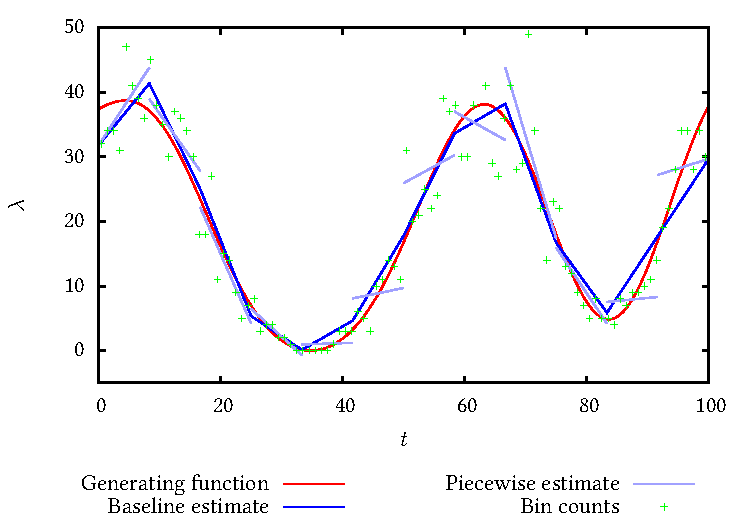
\includegraphics{images/pcbase}
    \caption{A comparison of the baseline and piecewise estimates on the same
    function. Note how the baseline estimate passes through the midpoint of the
    disjoint piecewise estimates at the breakpoints.}
    \label{fig:basecomp}
    \end{figure}
    \end{comment}
    
    This extension of IWLS produces piecewise disjoint estimates of the rate
    function. In order to produce the piecewise continuous functions that we
    require, we adjust the estimate in each sub-interval. We define breakpoints
    as the point in time where one sub-interval ends and another begins. There
    are $R=L-1$ breakpoints $r$, where L is the number of sub-intervals. At each
    breakpoint, the values of the two function estimates $f$ before adjustment
    are computed, and the midpoint $m$ is calculated.

    \begin{equation} 
    m_i = \frac{f_{i}(r_i) + f_{i+1}(r_i)}{2},\quad 0\leq i < R
    \end{equation}

    At the start of the first and end of the last sub-intervals the original
    function value is used as the midpoint. Each sub-interval is now represented
    by a point $p$ at the start and $q$ at the end, each with an $x$ and $y$
    coordinate. With these points, we can recalculate each sub-interval estimate
    $f$ of the form $y=\hat{a}+\hat{b}x$ by replacing $y$ with $p_y$ and $x$
    with $p_x$, and recalculating the gradient $\hat{b}$ and intercept $\hat{a}$
    with

    \begin{align} 
    \hat{b} &= \frac{q_y-p_y}{q_x-p_x}\\
    \hat{a} &= p_y - \hat{b}\cdot p_x 
    \end{align}

    This adjustment produces the desired piecewise continuous function by having
    the values of the estimates from the previous and next sub-interval have the
    same value at the breakpoint.
\subsection{Kernel Density Estimation}
\label{sec-4.2}

   The second function estimation method implemented was a kernel density
   estimator, which uses \emph{kernels} to estimate the probability density of a
   random variable. A kernel is simply a weighting function, which affects how
   much a given sample is considered when constructing the function
   estimate. Since the photon stream data is assumed to be generated by a source
   whose variability is defined by some random variable, the event times are a
   sample drawn from the PDF of that variable. We use a Gaussian kernel
   \begin{align}
   K(t,\mu)=e^{-(t-\mu)^2/2\sigma^2}
   \end{align}
   to estimate the PDF, centring a kernel at each photon arrival time $\phi_n$ by
   setting $\mu=\phi_n$. The width of the kernel depends on some fixed value
   $\sigma$. We perform a Gauss transform on the $N$ kernels, finding the
   contribution of all the kernels at $M$ points in time, from which we get an
   estimate $\hat{\lambda}(t)$ of the characteristic function.
   \begin{align}
   \hat{\lambda}(t_i) = \sum_{j=1}^N K(t_i,\mu_j), \quad i=1,\dots,M
   \end{align}
   Using a larger $M$ gives a higher resolution. Depending on the value of
   $\sigma$ used, $\hat{\lambda}(t)$ will be some multiple of the actual
   function $\lambda(t)$. Thus, the final step is to normalise
   $\hat{\lambda}(t)$. We split the stream data into $B$ bins with midpoints $b$
   and calculate the bin count $x$ for each. We start with the normalisation
   constant $\eta$ at a low value, and gradually increase it to some threshold,
   finding
   \begin{equation}\label{eq:normcalc}
   \sum_{i=1}^B
   \log\left(\frac{\phi^xe^{-\phi}}{x!}\right), \quad \phi=\eta\cdot\hat{\lambda}(b_i)
   \end{equation}
   for each value of $\eta$. The value of $\eta$ which maximises this sum of log
   Poisson PDFs is used to normalise $\hat{\lambda}(t)$ in subsequent
   computations. Figure \ref{fig:kde} shows an example of a kernel density
   estimate, and displays a weakness in the estimator. As one moves towards the
   start or end of the interval, fewer Gaussians make a noticeable contribution
   to the function calculation, resulting in a drop-off of the estimate.
\section{Time Delay Estimation}
\label{sec-5}

  Once we are able to estimate the characteristic function of photon streams, we
  can use these estimates to compute an estimate of the time delay between two
  streams. If the two streams come from the same source, then they should have
  the same characteristic function, but delayed by some value $\Delta$. Our
  estimates of the characteristic function will differ for both streams due to
  the fact that the number of photon arrivals in each bin will be different for
  each stream, but each should look relatively similar. In this section we
  present two methods for estimating the time delay between a pair of streams
  based on their function estimates.

  Both of the estimators work by starting $\Delta$ at $-\Delta_{\text{max}}$,
  and increment it by some step until reach $+\Delta_{\text{max}}$ is reached,
  using a metric to evaluate how good the estimate is with that value. It is
  important to note that the value of $\Delta_{\text{max}}$ defines the interval
  in which the metric is computed. The need for calculation only in some
  specific interval should be clear---if one function is shifted by $\Delta$,
  and both functions have the same time interval, then there will be an interval
  of length $\Delta$ at either end of the range in which only one of the
  function estimates has values. As such, the metric can only be computed in the
  overlapping area. Varying $\Delta$ changes the overlapping interval. Setting
  $\Delta=0$ minimises the value, and $\Delta=\pm\Delta_{\text{max}}$ maximises
  it. Performing calculations on different interval lengths would require the
  value of the metric for longer intervals to be scaled to that of the
  shortest. To make useful comparisons, we must perform calculations only on the
  interval in which the two functions overlap for all values of
  $\Delta$. Imposing this constraint means that the value of
  $\Delta_{\text{max}}$ can never exceed the interval length $T_{\text{est}}$ in which we are
  performing the estimate. We are left with the constraints
  $T_{\text{est}}=[t_0+\Delta_{\text{max}},
  T-\Delta_{\text{max}}],\,\Delta_{\text{max}}<T$ on the interval and the
  maximum value of $\Delta$.
\subsection{Area Method}
\label{sec-5.1}

   The first of the two methods uses a very simple metric to estimate the time
   delay. By taking the two function estimates, we can attempt to match up the
   two functions so that they ``fit together'' best. The goodness of fit can be
   determined by the area between the two functions $\hat{\lambda}_1$ and
   $\hat{\lambda}_2$, calculated by
   \begin{align}
   \begin{split}
   d(\hat{\lambda}_1,\hat{\lambda}_2)&=\int(\hat{\lambda}_1(t)-\hat{\lambda}_2(t+\Delta))^2\,dt\\
   &\approx\frac{1}{N}\sum_{i=1}^N(\hat{\lambda}_1(t)-\hat{\lambda}_2(t+\Delta))^2
   \end{split}
   \end{align}
   for each value of $\Delta$. Our estimate of $\Delta$ is set to the value at
   which $d(\hat{\lambda}_1,\hat{\lambda}_2)$ is minimised. Rather than using an
   integral to get the exact area between the functions, we use a less
   computationally expensive discrete approximation.
\subsection{PDF Method}
\label{sec-5.2}

   The second method of estimation is using probability density functions. As
   before, we guess a value of $\Delta$ between $-\Delta_{\text{max}}$ and
   $+\Delta_{\text{max}}$ and shift $\hat{\lambda}_2$ by that amount. However,
   we know that there must be a single characteristic function, and we want to
   see how well our estimate of that matches the bin counts in each stream. We
   make an ``average'' function $\bar{\lambda}$ by combining the two function
   estimates we have, $\hat{\lambda}_1$ and $\hat{\lambda}_2$ (which is shifted
   by $\Delta$).
   \begin{equation}
   \bar{\lambda}(t)=\frac{\hat{\lambda}_1(t)+\hat{\lambda}_2(t+\Delta)}{2}
   \end{equation}
   The point on $\bar{\lambda}$ at time $t$ is the midpoint between the values of
   the two estimates at that time. Once we have $\bar{\lambda}$, we can assign some
   score to the current estimate of the value of $\Delta$.
   \begin{align}
   \begin{split}
   \log P(S_A,S_B\mid\bar{\lambda}(t))=\sum_{t=\Delta_{\text{max}}}^{T-\Delta_{\text{max}}}&\log P(S_A(t)\mid \bar{\lambda}(t))\\
   &+ \log P(S_B(t+\Delta)\mid \bar{\lambda}(t))\\
   \end{split}
   \end{align}
   Here, we calculate the probability that the function $\bar{\lambda}$ is the
   characteristic function of the two streams $S_A$ and $S_B$. The streams are
   split into bins, and the log probability of the number of events in each bin
   given the value of $\lambda$ calculated for that bin is computed and summed
   over all bins, as in Equation \eqref{eq:normcalc}.

   The calculation of $\lambda$ is slightly more complicated than just taking
   its value at the midpoint of each bin. Since we are considering a number of
   events occurring in a given interval, we must consider the value of $\lambda$
   for the same interval. In order to do this, we use a discrete approximation
   of integrating $\lambda(t)$ over the interval.
   \begin{align}
   \lambda_{a,b}&=\int_a^b\lambda(t)\,dt
   \end{align}
   In the approximation $t$ is incremented by some finite step for each
   successive value. The smaller the value of the step the more accurate the
   approximation of $\lambda_{a,b}$ becomes. As with the previous estimator, the
   estimate is made in two stages, first with a coarse pass over the values of
   delta to compute an initial estimate, and then a finer second pass around the
   first estimated value in order to refine the estimate. 
\section{Experimental Results}
\label{sec-6}

\begin{itemize}
\item general explanation of the experiments performed
\item how was model selection done
\item what sort of data were experiments performed on
\end{itemize}
\section{System}
\label{sec-7}

\begin{itemize}
\item very brief explanation of the system features
\end{itemize}
\section{Conclusion}
\label{sec-8}

\begin{itemize}
\item some suggestions for extensions
    \printbibliography
\end{itemize}
$^{1}$ FOOTNOTE DEFINITION NOT FOUND: 1


\end{document}